% TO-DO:
% * slides to mention big achievements, 附件

\documentclass[16pt]{beamer}
% \geometry{papersize={5in,4.5in}}

\ifdefined\chinchin
\usepackage[CJKspace]{xeCJK}
%\setCJKmainfont[BoldFont=SimHei,ItalicFont=AR PL KaitiM GB]{Alibaba PuHuiTi}
\setCJKmainfont{Alibaba PuHuiTi}
\newcommand{\cc}[2]{#1}
\else
\newcommand{\cc}[2]{#2}
% \renewcommand{\baselinestretch}{0.8} 
\fi

%\usepackage{newtxtext,newtxmath}	% use Times Roman font
%\usepackage{newtxtext}
%\renewcommand{\familydefault}{\sfdefault}
\usefonttheme{serif}
\usefonttheme{professionalfonts}
%\setbeamertemplate{theorems}[numbered]
\setbeamertemplate{caption}{\insertcaption} 	% no `Figure' prefix before caption

\mode<presentation> {

%\usetheme{default}
%\usetheme{AnnArbor}
%\usetheme{Antibes}
%\usetheme{Bergen}
%\usetheme{Berkeley}
%\usetheme{Berlin}
%\usetheme{Boadilla}
%\usetheme{CambridgeUS}
%\usetheme{Copenhagen}
%\usetheme{Darmstadt}
%\usetheme{Dresden}
%\usetheme{Frankfurt}
%\usetheme{Goettingen}
%\usetheme{Hannover}
%\usetheme{Ilmenau}
%\usetheme{JuanLesPins}
%\usetheme{Luebeck}
\usetheme{Madrid}
%\usetheme{Malmoe}
%\usetheme{Marburg}
%\usetheme{Montpellier}
%\usetheme{PaloAlto}
%\usetheme{Pittsburgh}
%\usetheme{Rochester}
%\usetheme{Singapore}
%\usetheme{Szeged}
%\usetheme{Warsaw}

%\usecolortheme{albatross}
%\usecolortheme{beaver}
%\usecolortheme{beetle}
%\usecolortheme{crane}
%\usecolortheme{dolphin}
%\usecolortheme{dove}
%\usecolortheme{fly}
%\usecolortheme{lily}
\usecolortheme{orchid}
%\usecolortheme{rose}
%\usecolortheme{seagull}
%\usecolortheme{seahorse}
%\usecolortheme{whale}
%\usecolortheme{wolverine}		% Hofstra

%\setbeamertemplate{footline} % To remove the footer line in all slides uncomment this line
\setbeamertemplate{footline}[page number] % To replace the footer line in all slides with a simple slide count uncomment this line
\setbeamertemplate{navigation symbols}{} % To remove the navigation symbols from the bottom of all slides uncomment this line
}

\setbeamertemplate{headline}{}
% \setbeamersize{text margin left=1mm,text margin right=1mm} 
% \settowidth{\leftmargini}{\usebeamertemplate{itemize item}}
% \addtolength{\leftmargini}{\labelsep}
% \setbeamertemplate{enumerate subitem}{(\roman{enumii})}
% \setbeamertemplate{itemize items}[default]
\setbeamertemplate{items}[square]
\setbeamertemplate{enumerate items}[default]

\usepackage[backend=biber,style=numeric]{biblatex}
\bibliography{../../AGI-book}
% \renewcommand*{\bibfont}{\footnotesize}
\setbeamertemplate{bibliography item}[text]

\usepackage{graphicx} % Allows including images
\usepackage{tikz-cd}
\usetikzlibrary{decorations.pathmorphing}
% \usepackage{tikz}
\usepackage[export]{adjustbox}% http://ctan.org/pkg/adjustbox
\usepackage{verbatim} % comments
\usepackage[skins,theorems]{tcolorbox}

\usepackage{ulem}
\makeatletter
\newcommand{\cthickuline}[3][0.5pt]{%
	\UL@protected\def\temp@uline{\bgroup\markoverwith
		{\textcolor{#2}{\rule[-0.5ex]{2pt}{#1}}}\ULon}%
	\temp@uline{#3}%
}
\makeatother

% \usepackage{tikz-cd}  % commutative diagrams
% \newcommand{\tikzmark}[1]{\tikz[overlay,remember picture] \node (#1) {};}
% \usepackage{booktabs} % Allows the use of \toprule, \midrule and \bottomrule in tables
% \usepackage{amssymb}  % \leftrightharpoons
% \usepackage{wasysym} % frownie face
% \usepackage{newtxtext,newtxmath}	% Times New Roman font
% \usepackage{sansmath}

\let\oldtextbf\textbf
\renewcommand{\textbf}[1]{\textcolor{blue}{\oldtextbf{#1}}}
\newcommand{\emp}[1]{\textbf{\color{violet}#1}}

\newcommand{\vect}[1]{\boldsymbol{#1}}
\newcommand{\tab}{\hspace*{1cm}}
\newcommand*\confoundFace{$\vcenter{\hbox{\includegraphics[scale=0.2]{../../confounded-face.jpg}}}$}
\newcommand{\smiley}{$\vcenter{\hbox{\includegraphics[scale=0.05]{../../smiling-face.png}}}$}
\newcommand{\cubic}{\vcenter{\hbox{\includegraphics[scale=1]{../../cubic-symbol.png}}}}

\makeatletter
\renewcommand{\boxed}[1]{\fbox{\m@th$\displaystyle\scalebox{0.9}{#1}$} \,}
\makeatother

%----------------------------------------------------------------------------------------
%	TITLE PAGE
%----------------------------------------------------------------------------------------

\title[AGI and categorical logic]{{Paper: AGI from the perspectives of categorical logic and algebraic geometry}}
\author{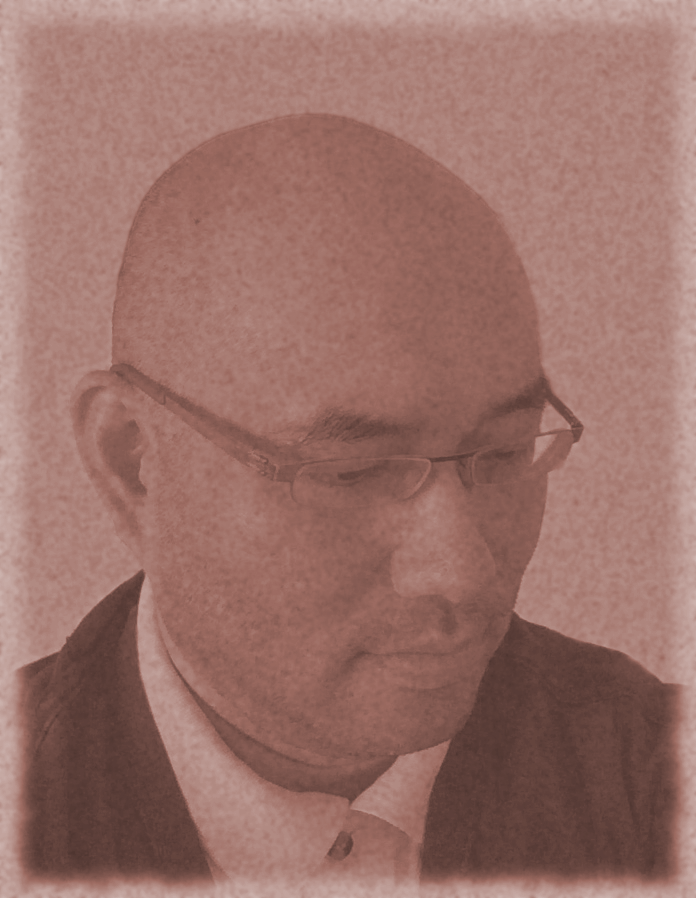
\includegraphics[scale=0.14]{John_Grothendieck.png} \\ \centering YKY}
\date{\today} % Date, can be changed to a custom date

\begin{document}

\addtocounter{page}{-1}
\begin{frame}[plain,noframenumbering]
\titlepage
\end{frame}

\addtocounter{page}{-1}
\begin{frame}[noframenumbering]
\frametitle{Contents}
\fontsize{10pt}{8}\selectfont
My paper was not very well-written, nor easy to understand.  That's not usually my style, but if I don't embellish the paper with some pretensions, it may not get published \smiley  \ \ In this presentation I try to explain my ideas more easily: \\

\begin{enumerate}[I]
	\item In the first part I try to explain how the theory of ``\textbf{No Free Lunch}'' and inductive biases is a basis for accelerating AGI (in particular the learning process).  This is based on an informal argument which I have difficulty making rigorous.
	
	\item In the second part I explain \textbf{categorical logic} (as the structure of logic), in particular the notion of ``fibrations'' which describe predicate logics.  But my conclusion is that fibrations are not very useful for accelerating learning, because it is actually isomorphic to the ``boring'' concatenation of tokens that we currently use in LLMs.
	
	\item The third part contains an idea that I discovered after submitting the paper, a kind of ``\textbf{algebraic-logic}'' neural network.  Algebra, algebraic geometry, and polynomials are powerful tools in mathematics with a long history, much older than Curry-Howard isomorphism and category theory.  They may offer more techniques to accelerate learning.
\end{enumerate}
\end{frame}

%----------------------------------------------------------------------------------------
%	PRESENTATION SLIDES
%----------------------------------------------------------------------------------------

\part{How does ``No Free Lunch'' guide us to accelerate AGI?}
\frame{\partpage}

\begin{frame}
\frametitle{The basic argument}
\begin{itemize}
	\item We know very little about how \textbf{AGI solutions} are distributed in the hypothesis space (ie parameter space of neural networks), but exploring this space is very expensive (= training large models)
	\item We know with some certainty that at least one AGI solution exists in the structural \textbf{sub-space} conforming to formal symbolic logic (the kind that humans are familiar with).
	\item By a probabilistic argument based on ``\textbf{ignorance}'' \footnote{similar to the argument we make to assign 1/6 to the rolling of a die}, it seems reasonable to confine our search within this sub-space rather than in other ``unknown'' regions.  But I'm not sure if this argument is sound, perhaps the reader can help validate or disprove it?
\end{itemize}
\end{frame}


\begin{frame}
\frametitle{The hypothesis space, ie. the space of AGIs}
\begin{itemize}
	\item In deep learning, our hypothesis space $\Theta$ = neural networks = parameter space = weight space = $\mathbb{R}^n$ or $[0,1]^n$ if truncated.

	\item It looks like this (left):
	\begin{equation}
	\Theta = \vcenter{\hbox{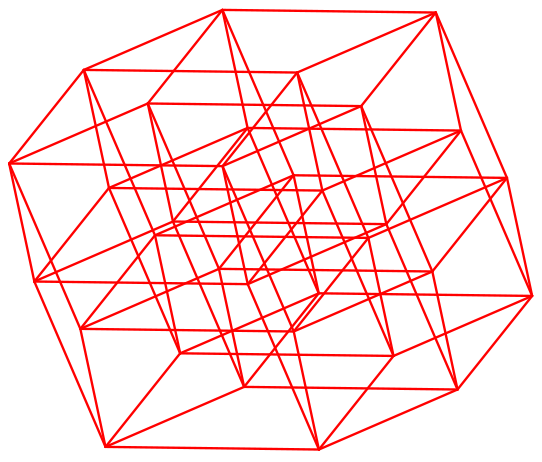
\includegraphics[scale=0.18]{hypercube.png}}} \qquad \qquad
	\vcenter{\hbox{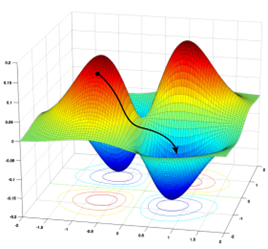
\includegraphics[scale=0.4]{error-landscape.png}}}
	\nonumber
	\end{equation}

	\item Imagine a loss function as sitting above the hypercube;  We seek to minimize it by \textbf{gradient descent}.
	
	\item When people visualize gradient descent, they tend to think of the above figure (right), but in practice, the ``ups and downs'' along one dimension is \textit{dominated} (overshadowed) by the sheer number of dimensions.
\end{itemize}
\end{frame}

\begin{frame}
\frametitle{The distance metric in gradient descent}
\begin{equation}
\Theta = \vcenter{\hbox{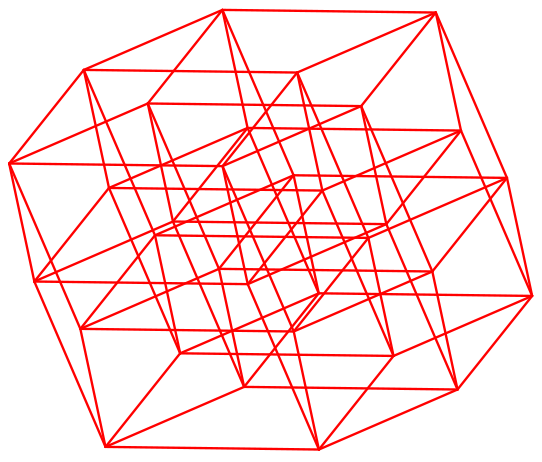
\includegraphics[scale=0.15]{hypercube.png}}}
\nonumber
\end{equation}
\begin{itemize}
	\item Training large models is costly.  We want to measure the cost of training neural networks by measuring the \textbf{size} of the hypothesis space $\Theta$ that we're searching.
	
	\item Gradient descent works by $\nabla_\Theta = \sum \frac{\partial}{\partial\theta_i}$.  Each step is a ``delta'' move in the parameter space $\Theta$.

	\item The distance metric we can use in the space $\Theta$ is the \textbf{Euclidean} one given by $ds^2 = d\theta_1^2 + d\theta_2^2 + ...$.
	
	\item So the \textbf{area} of parameter space measured by Euclidean metric is an estimation of how long it may take to converge to an AGI solution.
\end{itemize}
\end{frame}

\begin{frame}
	\frametitle{Unreasonable effectiveness of gradient descent}
	
	\begin{columns}
		\begin{column}{0.8\textwidth}
			\begin{itemize}
			\item Gradient descent can keep going down \textit{for a long time} as there are millions of dimensions.
			\item The ``unreasonable'' effectiveness of gradient descent in deep learning is currently our most powerful weapon to solve the AGI problem.  \\
			Its explanation is likely very difficult, as it hinges on the P =? NP problem.
			\end{itemize}
		\end{column}

		\begin{column}{0.2\textwidth}  %%<--- here
			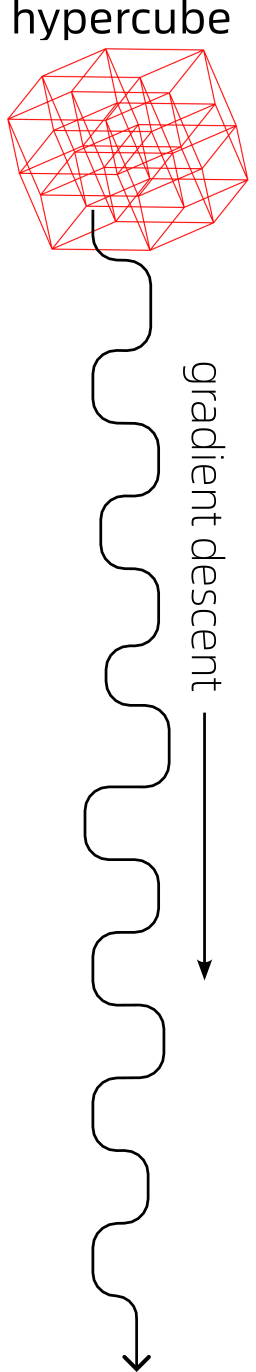
\includegraphics[scale=0.45]{gradient-descent-from-hypercube.png}
		\end{column}
	\end{columns}
\end{frame}

\begin{frame}
\frametitle{Finding an intelligent structure and filling it with intelligent knowledge}
\fontsize{10pt}{8}\selectfont
\begin{itemize}
	\item Symmetry allows us to restrict searching to a particular \textbf{sub-space} of the parameter space:
	\begin{equation}
	\vcenter{\hbox{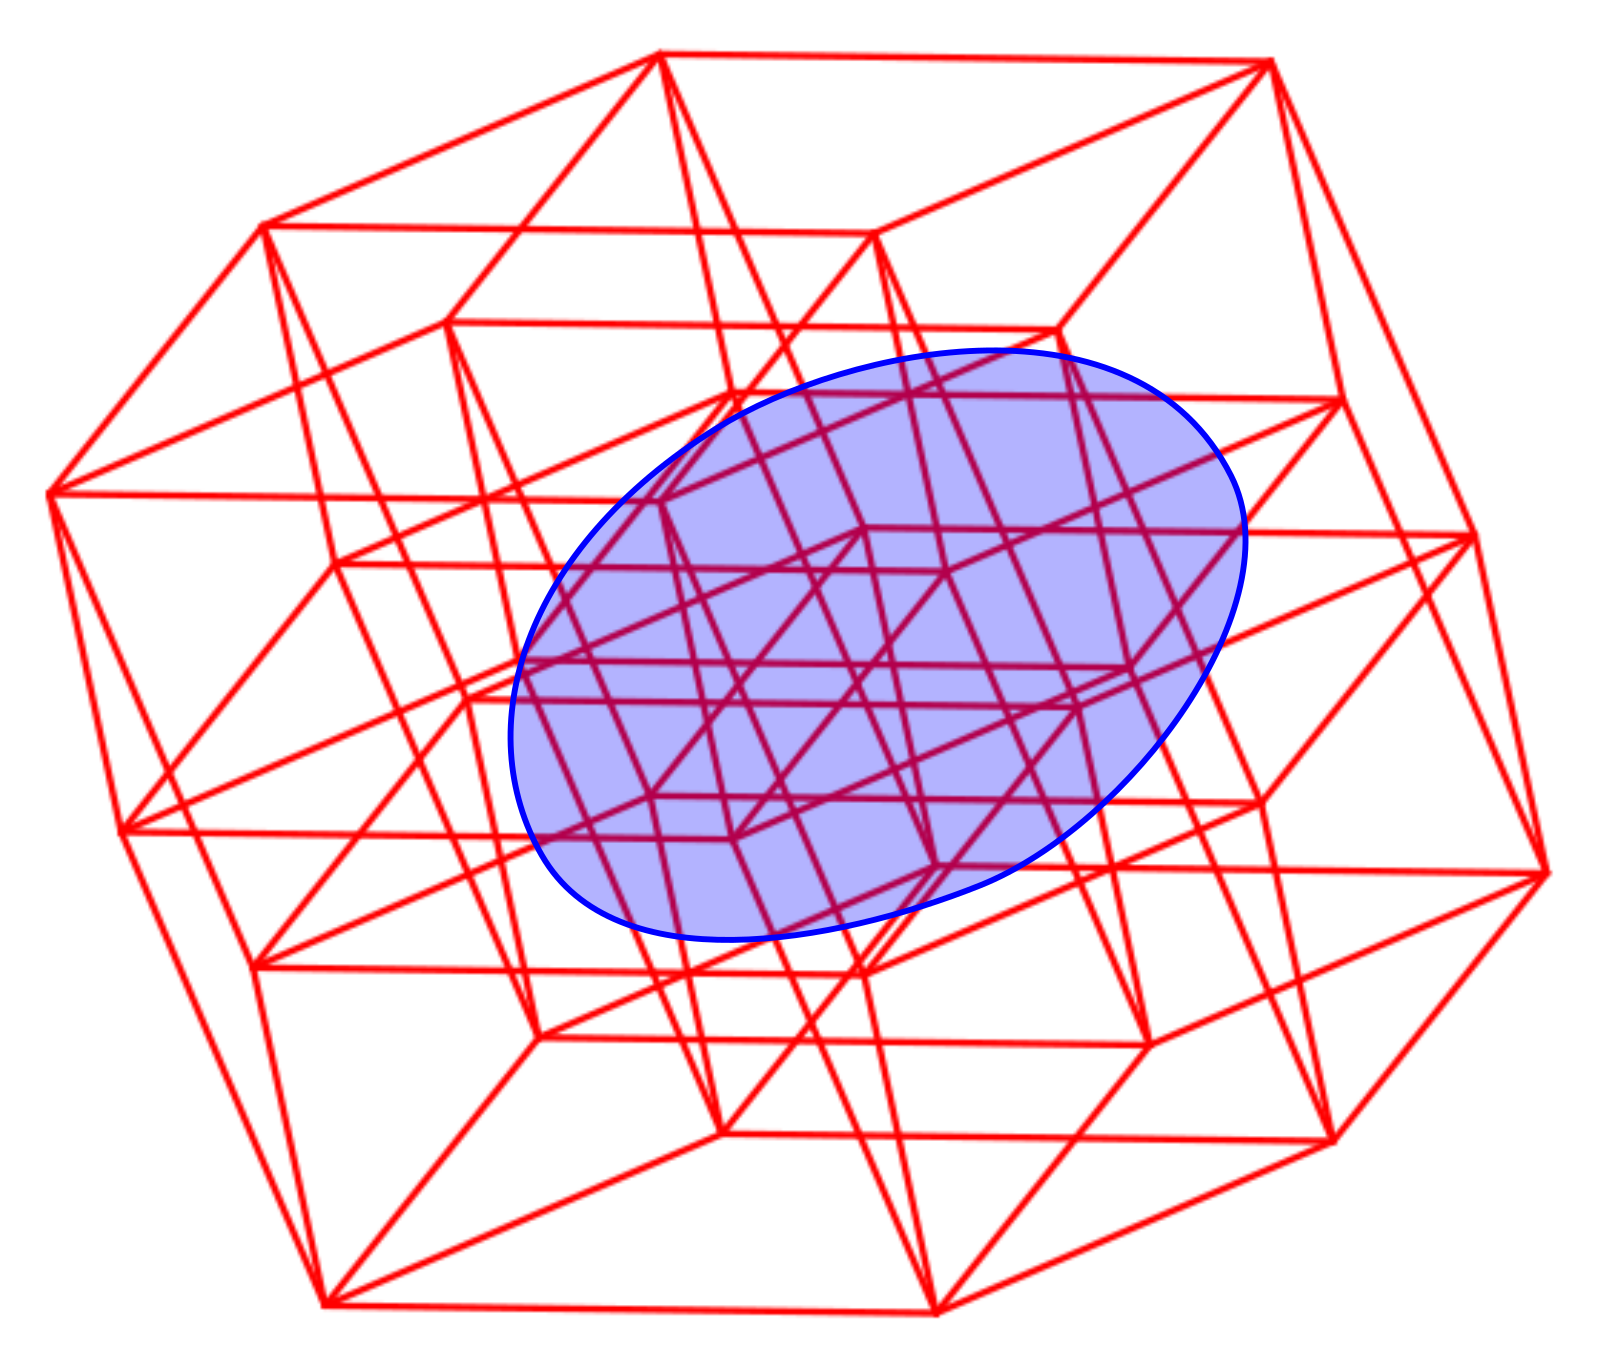
\includegraphics[scale=0.4]{subspace-of-hypercube.png}}}
	\nonumber
	\end{equation}
	
	\item After restricting to the right \textbf{structure}, we still need gradient descent to search for the right \textbf{knowledge}:
	\begin{equation}
	\vcenter{\hbox{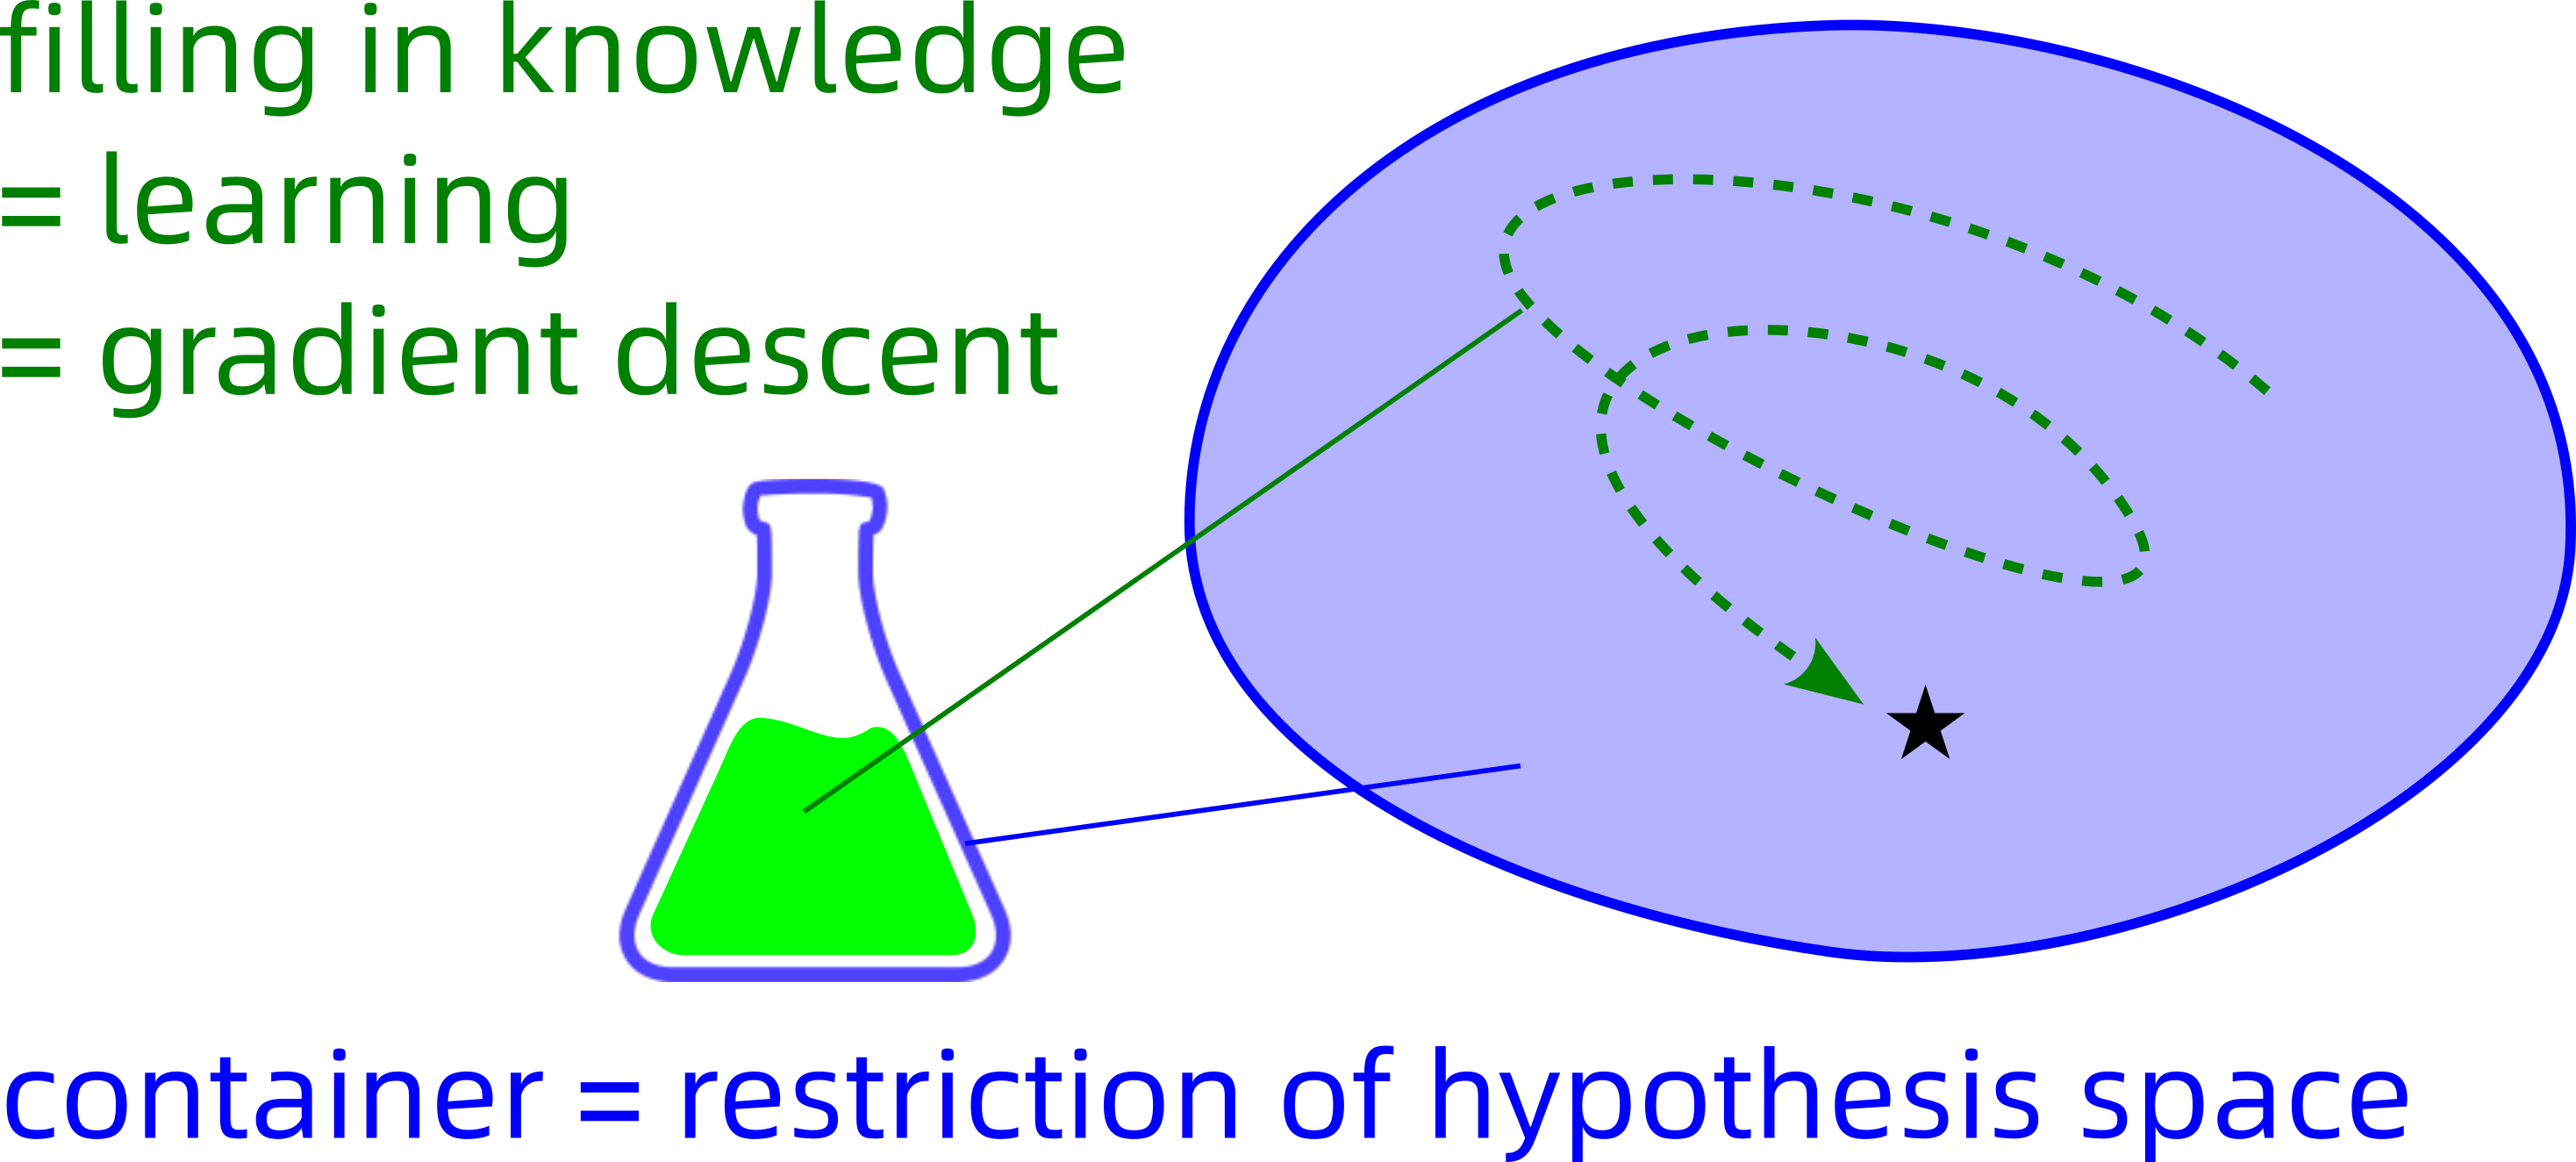
\includegraphics[scale=0.5]{structure-finding-vs-learning.png}}}
	\nonumber
	\end{equation}
	The parameter space represents both structure and knowledge.
\end{itemize}
\end{frame}

\begin{frame}
\frametitle{The hypothesis space has plenty of ``dumb structures''}
\begin{itemize}
	\item It seems that dumb learning-machine structures (animals) are more common than smart ones
\end{itemize}

\centering
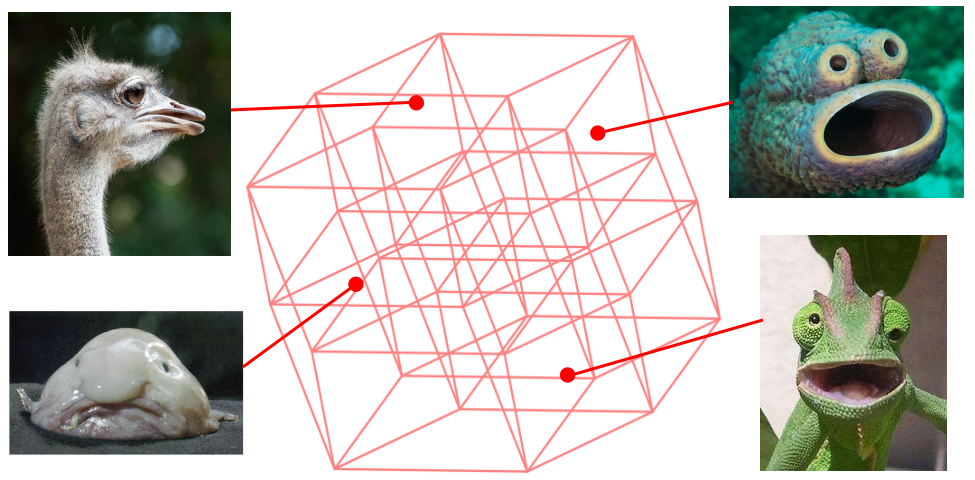
\includegraphics[scale=0.35]{dumb.png}
\end{frame}

\begin{frame}
	\frametitle{Even if we have found an intelligent structure, it may still contain lots of ``dumb knowledge'' in that sub-space}
\begin{itemize}
	\item It also seems that dumb knowledge is more common than smart knowledge
\end{itemize}

\centering
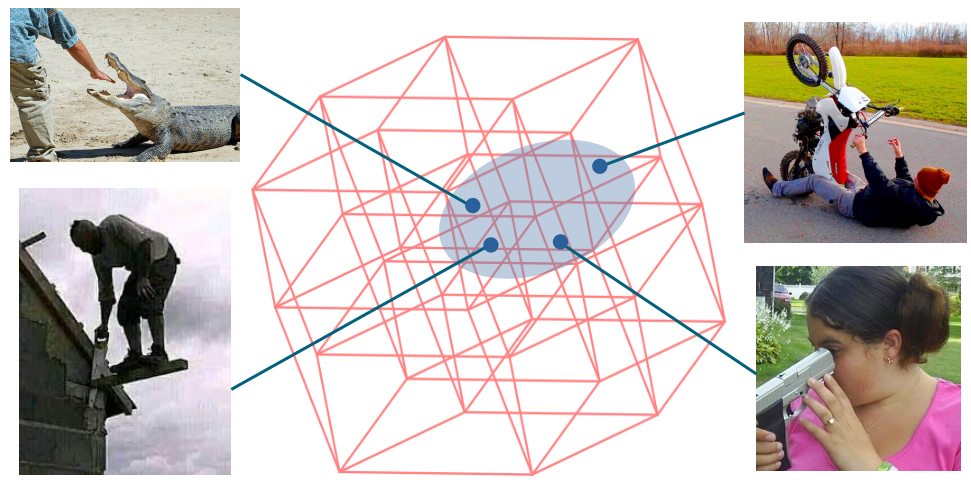
\includegraphics[scale=0.35]{dumb-behavior.png}
\end{frame}

\begin{frame}
\frametitle{Motivating example: symmetric neural networks}
\fontsize{10pt}{8}\selectfont
\begin{itemize}
	\item Now we turn to an artificial example where the No Free Lunch strategy can be proven to work.
	\item Permutation symmetry or commutativity ($ab = ba$) is the best-known symmetry in mathematics
	\item The input space, as a hypercube, is symmetric under exchange of vertices. The \textbf{fundamental domain} of this symmetry is one \textit{corner} of the hypercube:
	\begin{equation}
	\vcenter{\hbox{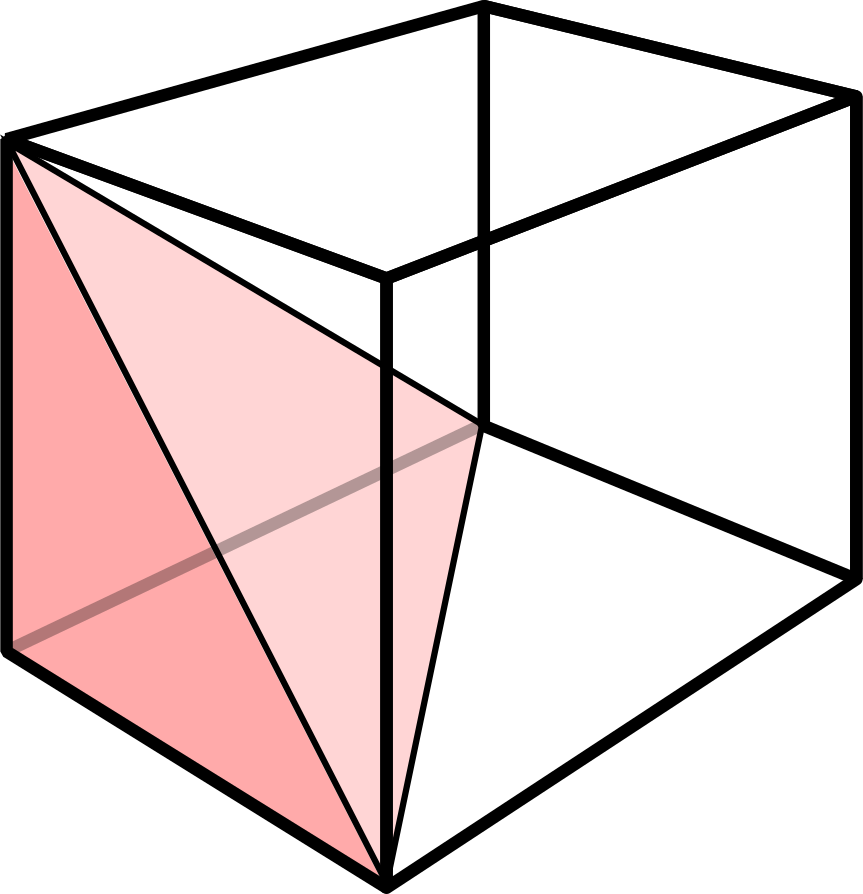
\includegraphics[scale=0.6]{cube-corner.png}}}
	\nonumber
	\end{equation}
	(Note that this hypercube is the \textit{input} space, not the mapping / hypothesis space)
	\item Building a symmetry into a neural network may seem a daunting task, but recent research shows that merely \textbf{projecting} all data points to the fundamental domain has the same effect as achieving symmetry \cite{Aslan2023}.
\end{itemize}
\end{frame}

\begin{frame}
	\frametitle{Motivating example: symmetric neural networks (2)}
	\begin{itemize}
		\item If we restrict to binary logic, the total number of Boolean functions in $n$ variables is $2^{2^n}$ whereas the number of \textbf{symmetric} Boolean functions is $2^{n+1}$.  So we clearly see an \textit{exponential} reduction in the size of the hypothesis space.
		
		\item Tantalizingly, the \textbf{Transformer} also has this permutation symmetry, and researchers have proposed that Transformers are capable of performing \textit{syntactic} manipulations similar to those in proofs of symbolic / predicate logic.
		
		\item We can further relax the restriction of binary logic to $k$-ary logic, ie, increase the number of lattice points in the hypercube, and the above analysis still holds qualitatively.  In the limit, this seems to apply to \textbf{smooth functions} as well.
	\end{itemize}
\end{frame}

\part{Categorical logic, and fibrations in particular}
\frame{\partpage}

\begin{frame}
\frametitle{Curry-Howard isomorphism}
Many readers are already familiar with this, so I'll just highlight some interesting points...
\begin{itemize}
	\item The starting point of the Curry-Howard isomorphism is the following correspondence:
	\begin{equation}
		\boxed{implication in logic} A \rightarrow B \qquad A \stackrel{f}{\rightarrow} B \; \boxed{function in type theory}
		\nonumber
	\end{equation}
	\item An example in type theory: ``\textbf{currying}'' means to convert a 2-argument function into a single-argument function which returns another function, ie. $f(x,y) = (g(x))(y)$.  \\
	The types of $f$ and $g$ are equivalent, ie, $X \rightarrow (Y \rightarrow Z) \simeq (X \times Y) \rightarrow Z$. \\
	If we treat the above as logic it becomes: $X \rightarrow (Y \rightarrow Z) \equiv (X \wedge Y) \rightarrow Z$.  One can verify this is a valid logic formula.
	\item This and other amazing coincidences led us to believe that CHI has some deep truth in it.
\end{itemize}
\end{frame}

\begin{frame}
\frametitle{Categorical logic \oldtextbf{clashes} with algebraic logic}
\fontsize{10pt}{8}\selectfont
	\begin{itemize}
	\item The late Joachim Lambek proposed a ``trinity'' between category theory, logic, and type theory \cite{Lambek1986}:
		\begin{equation}
		\begin{tikzcd}[row sep=1.5em,ampersand replacement=\&]
			\& \boxed{category theory} \arrow[dr,dash] \\
			\boxed{logic} \arrow[ur,dash] \arrow[rr,dash,"Curry-Howard"] \&\& \boxed{type-theory}
		\end{tikzcd}
		\label{eqn:trinity}
		\end{equation}
	\item But the Curry-Howard approach seems, at least on the surface, \textit{incompatible} with the \textbf{algebraic logic} approach, for example:
		\begin{equation}
		\begin{tikzcd}[row sep=2em,ampersand replacement=\&]
		\parbox{2.2cm}{\centering $f: A \rightarrow B$ \boxed{type theory}} \arrow[dr,dash,red,squiggly,"incompatible"] \& \\
		 \parbox{1.5cm}{\centering $a \rightarrow b$ \boxed{logic}} \arrow[u,"Curry-Howard"] \arrow[r] \& \parbox{1.8cm}{\centering $a \oplus ab = 0$ \boxed{algebraic logic}}
		\end{tikzcd}
		\nonumber
		\end{equation}
	\item I have been working in the Curry-Howard direction because it feels more ``modern'' but lately I began to think the algebraic logic approach may have more potential for computational acceleration.
	\end{itemize}
\end{frame}

\begin{frame}
\frametitle{Definition of a \oldtextbf{fiber bundle}}
\begin{columns}[T]
	\column{0.99\textwidth}
	A \textbf{fiber bundle} is a tuple $\xi = (E, p, B, F)$:
	\begin{enumerate}[(i)]
		\item $E$ = \textbf{total space}
		\item $B$ = \textbf{base space}
		\item $F$ = a topological space called the \textbf{fiber} of $\xi$
		\item $\mathrel{\substack{E\\\downarrow \\B}  {\scriptstyle p}}$ is a continuous surjective map, called the \textbf{projection}
		\item for each point $b \in B$, the inverse image $p^{-1}(b) = F_b$, called \cthickuline[1.2pt]{red}{the \textbf{fiber over} $b$, is homeomorphic to $F$}
		\item $B$ has an opening covering $\{ U_a \}_{a \in A}$ such that for each $a \in A$, there is a homeomorphism: $\psi_a: U_a \times F \rightarrow p^{-1}(U_a)$.  \\
		If $F$ is a discrete space, then the structure $F \hookrightarrow E \stackrel{p}{\rightarrow} B$ is called a \textbf{covering} of $B$.
	\end{enumerate}
	
	The condition (vi) is just a re-phrase of (v) in the form of open sets, similar to the ``gluing'' together of charts in differential manifolds.  So the essential condition is (v).
	
	\column{0.01\textwidth}
	\hspace*{-3.5cm}
	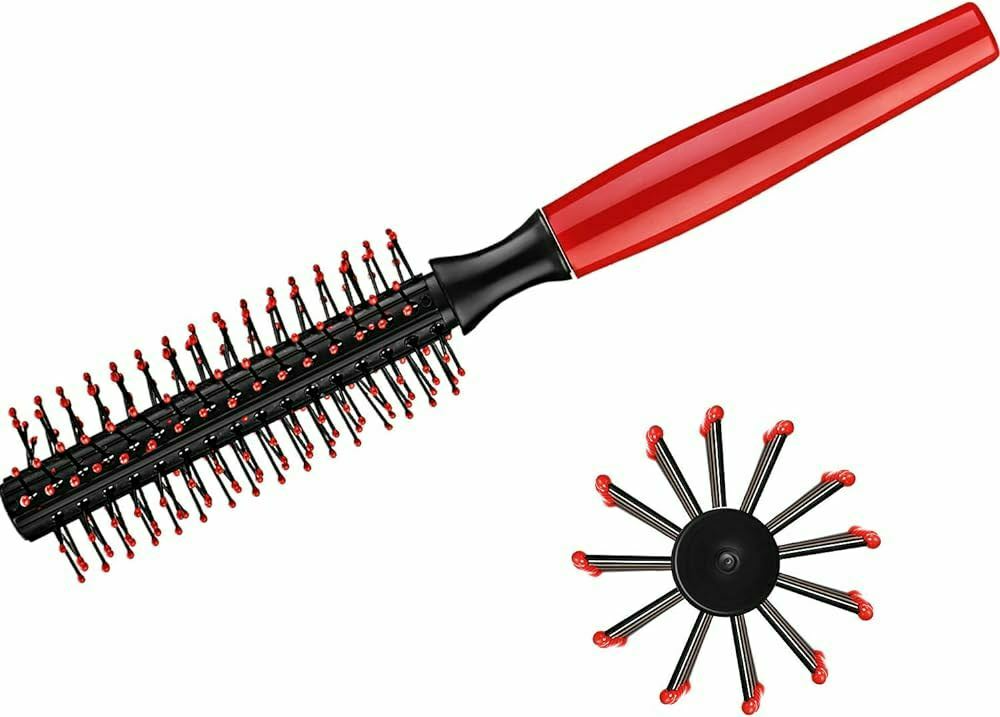
\includegraphics[width=3.5cm]{hair-brush.png}
\end{columns}
\end{frame}

\begin{frame}
\frametitle{The ``boring'' cross product}
\fontsize{10pt}{8}\selectfont
\begin{itemize}
	\item It was an anti-climax when I realized that fibrations do not offer a symmetry that reduces the size of the hypothesis space.
	\item An example of fibration for predicate logic is a relation $r(a,b)$ sitting above two entities $a,b$.
	\item If we treat the relation predicate and the entities as homogeneous atoms, ie. $r,a,b \in A$, then the term's type is just $A \times A \times A$, though it looks like $\substack{A\\\downarrow \\A \times A}$.
	\item Putting an atom above the other two does not change the fact that the whole type is isomorphic to $A \times A \times A$, and this Cartesian product of types is ``boring'' because it is basically the same as a sequence of ``tokens'' in LLM terminology:
	\begin{equation}
	.... \quad
	\tcbhighmath[boxrule=1pt,arc=6pt,colframe=black,shrink tight,extrude by=2mm]{token} \qquad
	\tcbhighmath[boxrule=1pt,arc=6pt,colframe=black,shrink tight,extrude by=2mm]{token} \qquad
	\tcbhighmath[boxrule=1pt,arc=6pt,colframe=black,shrink tight,extrude by=2mm]{token} \quad ....
	\nonumber
	\end{equation}
	which we have been using all the time.
	\item If we do not endow the fibration with more structure (such as a structure group $G$, giving rise to a $G$-bundle), then we are left with the boring Cartesian product, which does not offer any reduction / acceleration.
\end{itemize}
\end{frame}

\part{``Algebraic-logical'' neural networks}
\frame{\partpage}

\begin{frame}
\frametitle{Algebraic logic}
\begin{itemize}
	\item Traditionally, algebra (and algebraic geometry) is concerned with systems of \textbf{polynomials} over the ``classical'' number fields $\mathbb{R}$ or $\mathbb{C}$.  The polynomials are built upon addition and multiplication of numbers, that we're all familiar with.
	\item Propositional logic $(B, \wedge, \vee, \neg, \top, \bot)$ can be equated with \textbf{Boolean rings} $(B, \cdot, \oplus, -(), 0, 1)$, with ring multiplication identified as $\wedge$ and ring addition identified as symmetric difference (``XOR'').
	\item As predicate logic involves more operators (eg. $\forall$ and $\exists$), the classical algebra of numbers seems inadequate to represent them.
	\item For example, \textbf{cylindric algebra}\footnote{see Wikipedia for a quick intro} has additional operations $\mathsf{c}_i$ (cylindrification) and $\mathsf{Id}_{ij}$ (diagonal).
	\item Notice that algebra does not appear in the ``trinity'' (\ref{eqn:trinity}).  The Curry-Howard approach is not directly related to algebraic logic.
\end{itemize}
\end{frame}

\begin{frame}
\centering
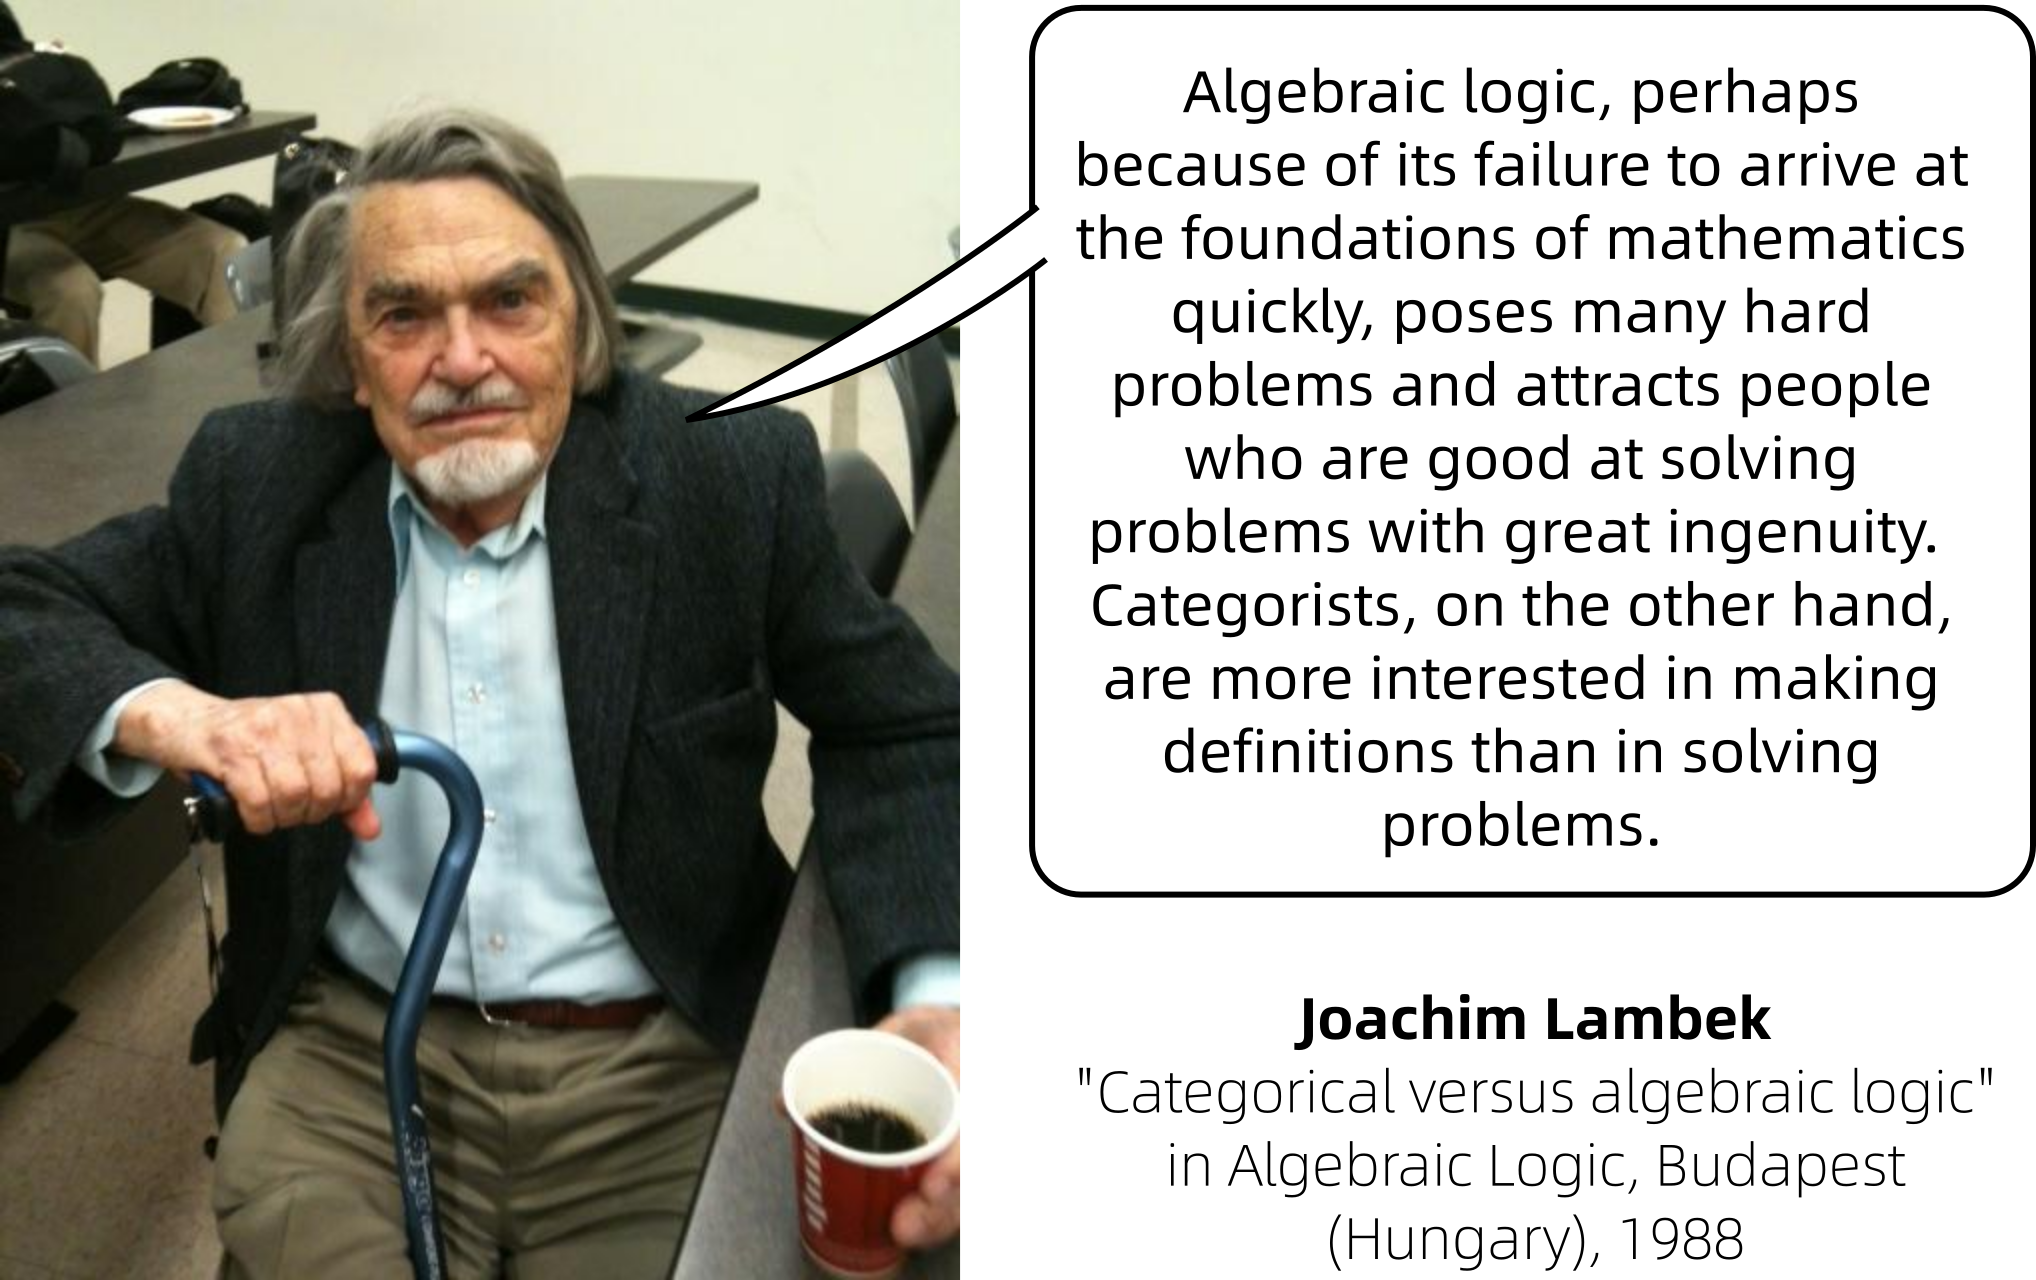
\includegraphics[scale=0.45]{Lambek-quote.png}
\end{frame}

\begin{frame}
\frametitle{Neural networks with polynomial activation functions}
\fontsize{10pt}{8}\selectfont
\begin{itemize}
	\item This is the basic setup of an auto-encoder which is the common setting for all current LLM models:
	\begin{equation}
	\vcenter{\hbox{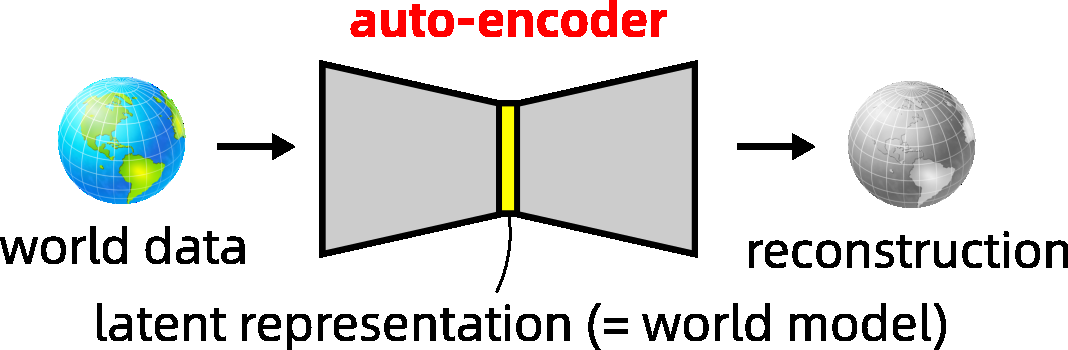
\includegraphics[scale=0.35]{auto-encoder.png}}}
	\nonumber
	\end{equation}

	\item The predictor / model can be construed as a logical \textbf{knowledge-base} (KB) making inferences:
	\begin{equation}
	\begin{tikzcd}[row sep=0em,column sep=5em,ampersand replacement=\&,| /.tip = {Bar[scale=2]}]
		\boxed{input state} \; \Gamma \arrow[r, |-, "\mbox{\tiny KB}"] \& \Delta \; \boxed{new conclusion} \\
		\Gamma \arrow[r,"\mbox{\tiny deep NN}", "\mbox{\tiny LLM / GPT / etc}"'] \& \Delta
	\end{tikzcd}
	\nonumber
	\end{equation}

	\item A neural network is composed of multiple layers:
	\begin{equation}
	\vcenter{\hbox{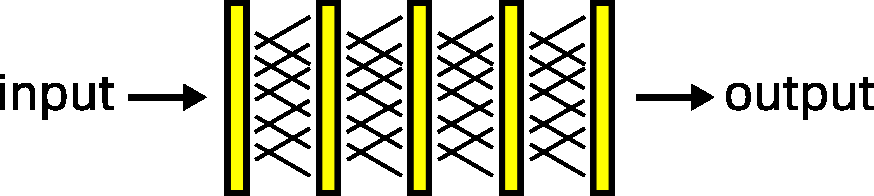
\includegraphics[scale=0.35]{NN-with-layers.png}}}
	\nonumber
	\end{equation}

	\item We can replace the activation functions with \textbf{polynomials}, creating ``\textbf{algebraic}'' neural networks.  Pushing \textbf{Curry-Howard} to its extreme, perhaps each layer of algebraic NN can be identified as a logical KB?
\end{itemize}
\end{frame}

\begin{frame}
\frametitle{One layer of neural network as a polynomial function}
\fontsize{10pt}{8}\selectfont
\begin{itemize}
	\item Andr\'{e}ka-N\'{e}meti \cite{Andreka2021} developed a \textbf{general framework} for studying algebraic logic, based on model-theoretic semantics.  A logic is $\langle F, M, mng, \vdash, \Vdash \rangle$ where $F$ = set of formulas, $M$ = class of models or possible worlds, $mng$ = meaning function: $F \times M \rightarrow \mathrm{Sets}$, $\vdash$ = syntactic provability, $\Vdash$ = semantic consequence, usually defined via $mng$.
	
	\item For example, in first-order logic, $mng(\psi)$ = set of all \textbf{evaluations} of variables $\vec{x}$ such that the formula $\psi(\vec{x})$ is satisfied in $\mathfrak{M} \in M$.

	\item For our purpose, let's start with a simple logic formula: $\forall x. P(x) \rightarrow Q(x)$.  It can be implemented in \textbf{vector-matrix form}:
	\begin{gather}
	\begin{matrix} \cubic \\ \cubic \end{matrix}
	\begin{pmatrix} P \\ x \end{pmatrix}
	\begin{pmatrix} M \\ \mathrm{Id} \end{pmatrix}
	= \begin{pmatrix} Q \\ x \end{pmatrix}
	\nonumber
	\end{gather}
	where $\cubic$ = element-wise activation function (polynomial), $M$ = transformation matrix.
	
	\item This is a bit tricky because our algebraic logic include terms that appear as input-output objects, as well as \textbf{maps} between such objects.  But the Andr\'{e}ka-N\'{e}meti framework is still applicable in essence.
\end{itemize}
\end{frame}

\begin{frame}
\frametitle{How does it help to accelerate learning?}
\begin{itemize}
	\item I just newly discovered this and need more time to explore.
	
	\item What we have here is quite interesting: on the one hand, a deep neural network capable of \textbf{gradient descent};  on the other hand it is also an algebraic logic.
	
	\item Our goal remains the same: to accelerate learning.  
\end{itemize}
\end{frame}

\begin{frame}
\frametitle{References}
\cc{多谢收看}{Thanks for watching} \smiley \vspace{1cm}
\printbibliography
\end{frame}

\end{document} 